\documentclass[11pt,a4paper]{article}
\usepackage[utf8]{inputenc}
\usepackage[T1]{fontenc}
\usepackage{geometry}
\usepackage{amsmath,amsfonts,amssymb}
\usepackage{lmodern} % scalable fonts for microtype
\usepackage{hyperref}
\usepackage{listings}
\usepackage{xcolor}
\usepackage{booktabs}
\usepackage{float}
\usepackage{fancyhdr}
\usepackage{titlesec}
\usepackage{enumitem}
\usepackage{tikz}
\usepackage{csquotes}
\usepackage{natbib}
\usepackage{minted}

% Page setup
\geometry{margin=2.5cm}
\setlength{\parskip}{0.6em}
\setlength{\parindent}{0pt}

% Header and footer
\pagestyle{fancy}
\fancyhf{}
\fancyhead[L]{Medium Mining}
\fancyhead[R]{\thepage}
\renewcommand{\headrulewidth}{0.4pt}
\setlength{\headheight}{14pt}

% Section formatting (more academic look)
\titleformat{\section}{\large\bfseries}{\thesection}{0.75em}{}
\titleformat{\subsection}{\normalsize\bfseries}{\thesubsection}{0.6em}{}
\titleformat{\subsubsection}{\normalsize\itshape}{\thesubsubsection}{0.5em}{}

% Code listing setup
\definecolor{codegreen}{rgb}{0,0.5,0}
\definecolor{codegray}{rgb}{0.5,0.5,0.5}
\definecolor{codepurple}{rgb}{0.58,0,0.82}
\definecolor{backcolour}{rgb}{0.97,0.97,0.95}
\definecolor{mediumpurple}{HTML}{5038A5}
\definecolor{mediumblue}{HTML}{005F99}

\lstdefinestyle{mystyle}{
    backgroundcolor=\color{backcolour},
    commentstyle=\color{codegreen},
    keywordstyle=\color{mediumblue},
    numberstyle=\tiny\color{codegray},
    stringstyle=\color{codepurple},
    basicstyle=\ttfamily\footnotesize,
    breaklines=true,
    captionpos=b,
    keepspaces=true,
    numbers=left,
    numbersep=5pt,
    showstringspaces=false,
    tabsize=2
}
\lstset{style=mystyle}

% Hyperlinks
\hypersetup{
    colorlinks=true,
    linkcolor=mediumpurple,
    citecolor=mediumblue,
    urlcolor=mediumblue,
    pdftitle={Comparative Analysis of Paid and Free Articles on Medium.com},
    pdfauthor={Moritz Enderle}
}

% Custom commands
\newcommand{\todo}[1]{\textcolor{red}{\textbf{TODO:} #1}}
\newcommand{\code}[1]{\texttt{#1}}
\newcommand{\important}[1]{\textbf{#1}}

\title{\Huge\bfseries Comparative Analysis of Paid and Free Articles on Medium.com}
\author{Florian Eder, Moritz Enderle}

\date{\today}

\begin{document}
\maketitle
\thispagestyle{empty}

\newpage
\tableofcontents
\newpage

\section*{Abstract}
\addcontentsline{toc}{section}{Abstract}
This report presents a comparative analysis of paid and free articles on Medium.com. Using a custom data acquisition pipeline, we collected a dataset of articles and performed statistical analysis to identify key differences in content characteristics, engagement metrics, and author behaviors between paid and free publications.

\section{Data Acquisition}

There is currently no publicly available dataset of articles on Medium.com we could use for our analysis. 
The next best option would have been a Medium.com API, but this does not exist.
Therefore, we had to build a custom data acquisition pipeline to scrape articles from Medium.com, focusing on both paid and free content.

\subsection{Legal Considerations}

As this process involves web scraping, which is strictly prohibited by Medium's Terms of Service, we got in touch with Medium's legal department to clarify the situation and obtain permission for our academic project.

Although we received permission to proceed, we ensured our scraping methodology does not overload or negatively impact Medium's services. This includes:
\begin{itemize}
    \item Respectful crawling delays between requests
    \item Compliance with robots.txt directives where applicable
    \item Limiting the total number of scraped articles to a reasonable amount
\end{itemize}

All collected data is used exclusively for academic research purposes and will not be redistributed or commercialized.

\subsection{Page Discovery}

Traditional content discovery methods are mostly based around spiders crawling links from one page to another. However, this approach would introduce a significant bias, as most articles on Medium.com are linked only to other articles within the same field (e.g. technology articles link to other technology articles). This would lead to a dataset that is not representative of the overall article distribution on Medium.com.

This led us to discover Medium's sitemaps as a more suitable approach for page discovery. The main sitemap is located at \code{https://medium.com/sitemap/sitemap.xml} and contains references to 20440 individual sitemaps, each containing up to 7000 URLs. In total, this results in 32 million URLs [as of March 2025]. We completed the whole process over 6 hours with a Gaussian distributed delay with mean 0.05 seconds. From these URLs, we were able to filter out a portion of non-article URLs (e.g. user profiles, tag pages, etc.).
This finally resulted in 14702 individual sitemaps and a total of just over 30 Million URLs.

To impose structure on the crawl schedule we adopted the sitemap-provided priority scores as an initial ordering heuristic. From there we applied a “most-seen-first” policy: recommended-article links observed while rendering a page trigger incremental boosts to their target URLs' crawl priority. This feedback loop yields a balanced sampling across topical clusters while still emphasizing pages with demonstrably high visibility.

\begin{figure}[H]
    \centering
    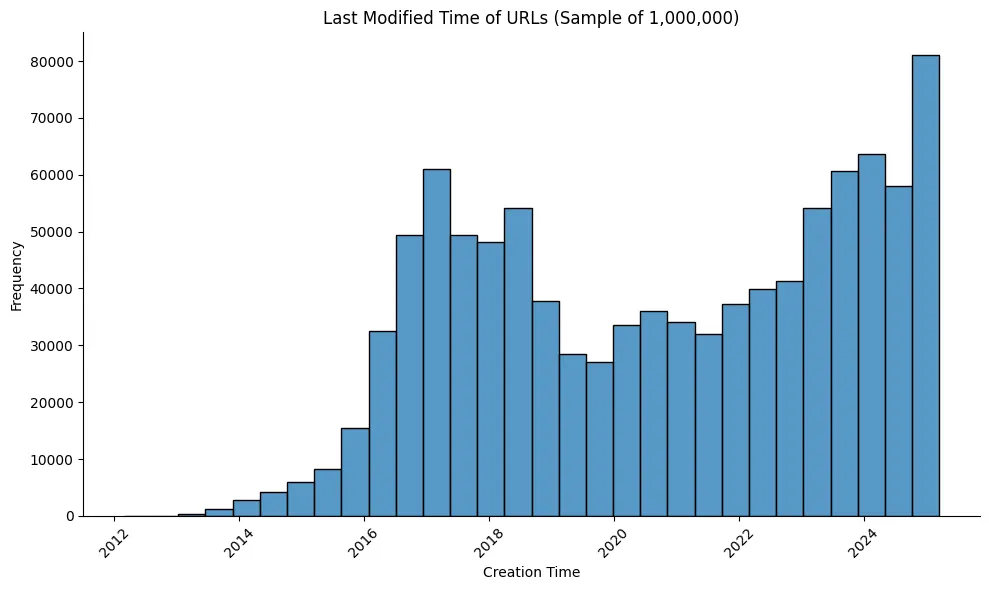
\includegraphics[width=0.8\textwidth]{images/Sitemaps_over_time.png}
    \caption{Distribution of Medium article last modification dates from sitemap data (2012-2024). The graph shows a peak in article creation around 2017, followed by a decline during the COVID-19 pandemic, and a notable resurgence since 2022, reflecting Medium's evolving content landscape and user engagement patterns.}
    \label{fig:sitemap_structure}
\end{figure}

\subsection{Scraping the Articles}

The articles on Medium.com are dynamically loaded using JavaScript, which means a simple HTTP request to fetch the HTML content is not sufficient. This is done mainly to optimize loading times and improve user experience. To overcome this issue, we used a headless browser to fully render the page before extracting the content. We employed Playwright, which provides a high-level API to control headless browsers. We integrated it into Python using the \code{playwright-python} package.

Due to the high number of articles to be scraped, we parallelized the process using multiple worker processes. Each worker operates independently, fetching URLs from the database, rendering the pages, and extracting the relevant data. 

We extracted most data directly from the rendered HTML using CSS selectors. However, some data points are embedded in JSON-LD structured data within the page, which we parsed to extract additional metadata. In order to capture the full comment thread, we programmed the scraper to simulate user interactions such as scrolling and clicking "see all responses" buttons. 

\todo{Diagram of the scraping pipeline}

\subsubsection*{Premium Content Access}

We fetched premium-only pages by logging in with a stored cookie as a JSON file. This allowed us to access member-only content while not having to deal with username and password authentication. During premium content scraping, we lowered the rates to avoid overloading the servers.

\subsection{Database Storage}

We stored data in DuckDB, a columnar database optimized for analytical queries. We designed the schema to include tables for sitemaps, URLs, articles, authors, and comments, with relationships maintained through foreign keys. This enables efficient querying for our comparative analysis.

\begin{figure}[H]
    \centering
    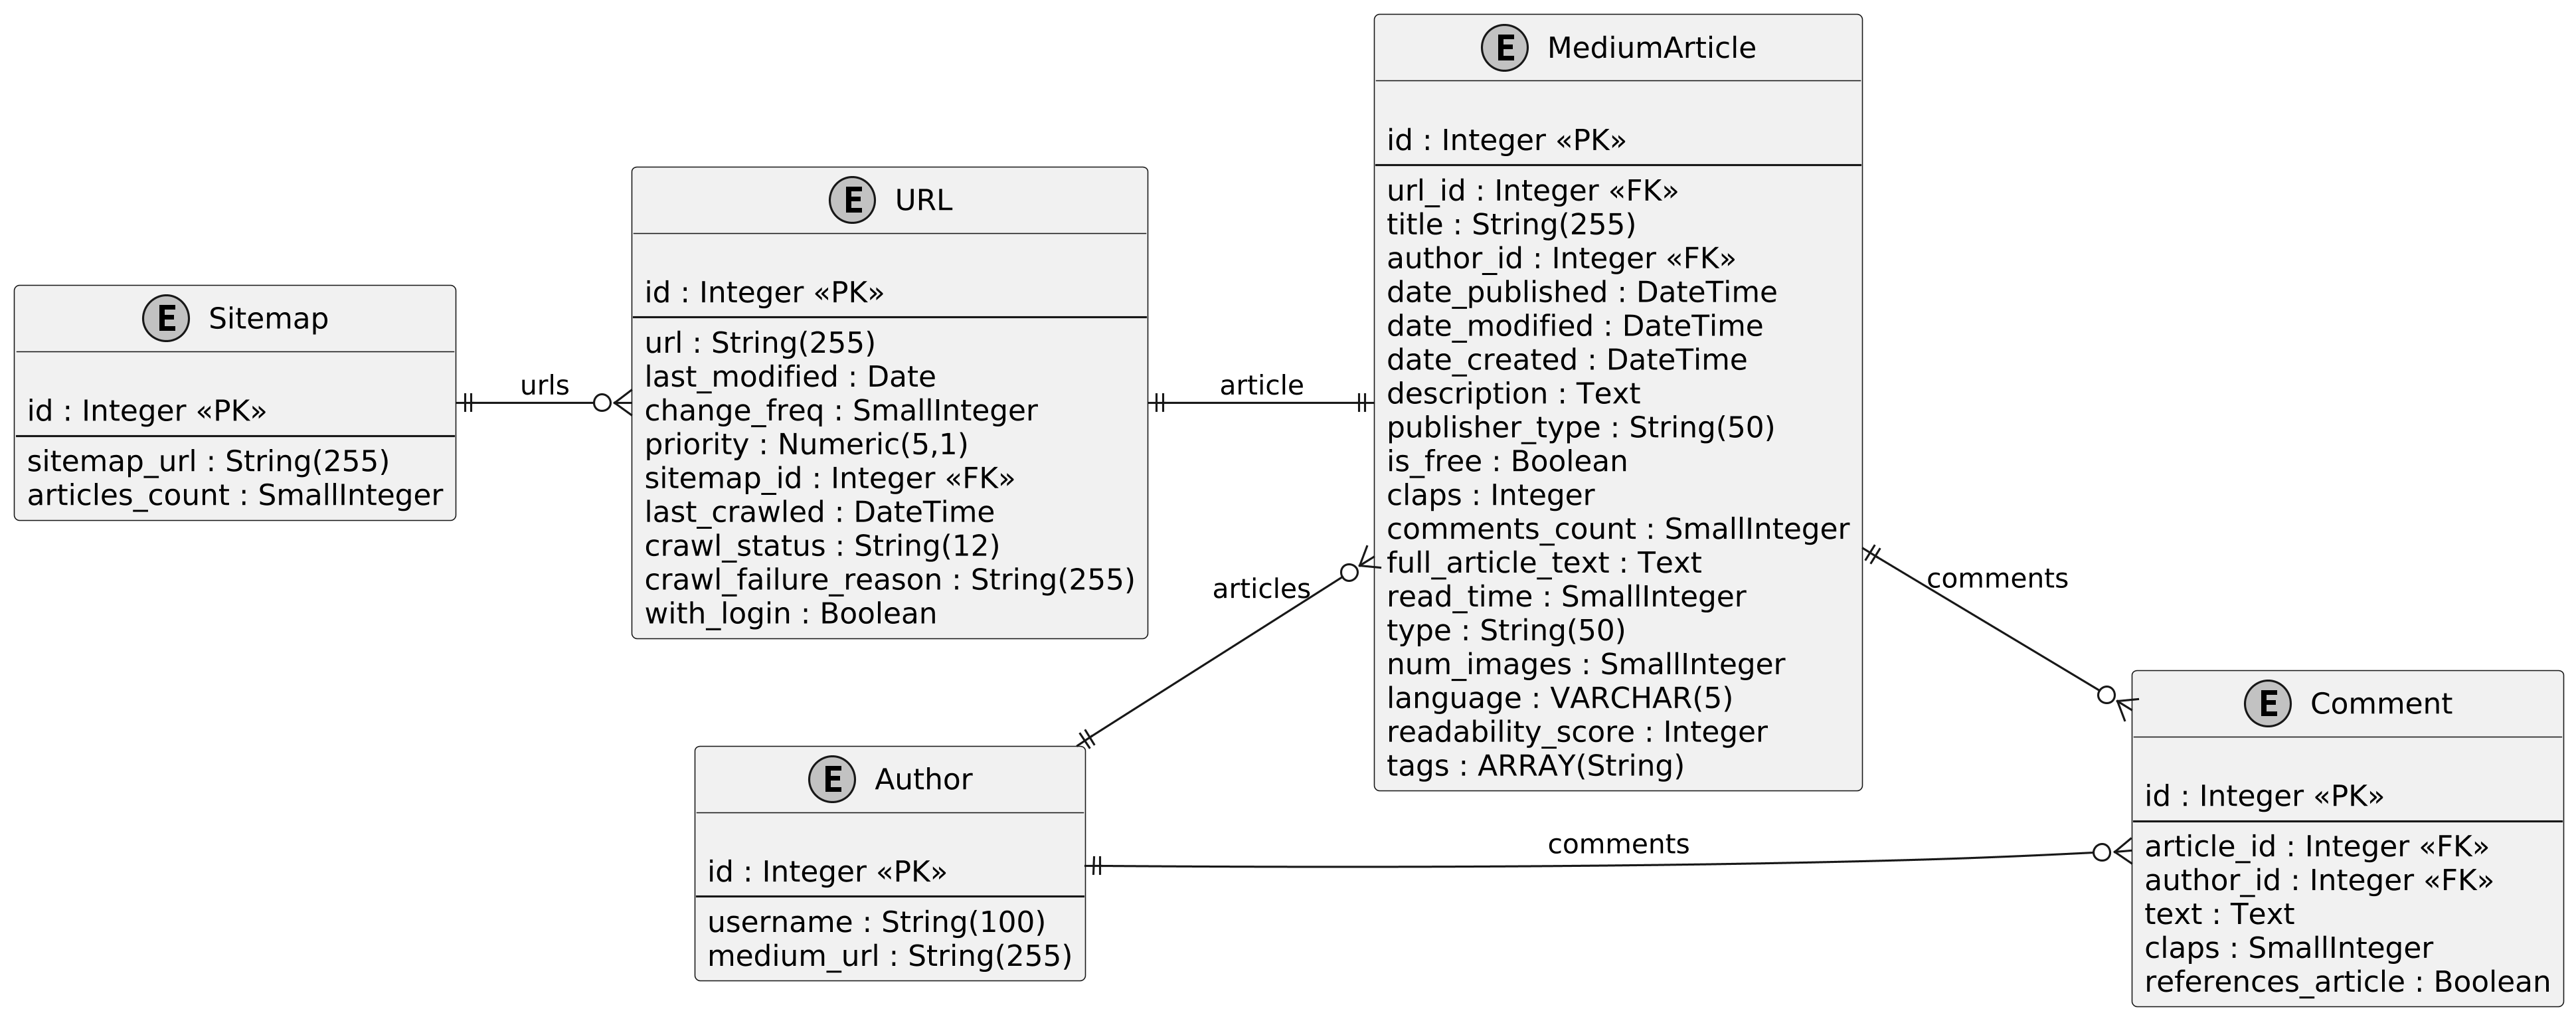
\includegraphics[width=\textwidth]{images/ER.png}
    \caption{Entity-relationship diagram of the scraping data model.}
\end{figure}

\subsection{Monitoring}

We implemented telemetry to track scraping health via structured worker logs aggregated into daily roll-ups for latency, error, and retry trends. We also configured the pipeline to push batch metrics to Weights \& Biases such as success ratios, premium hit rates, and fed into dashboards with alert thresholds.

\begin{figure}[H]
    \centering
    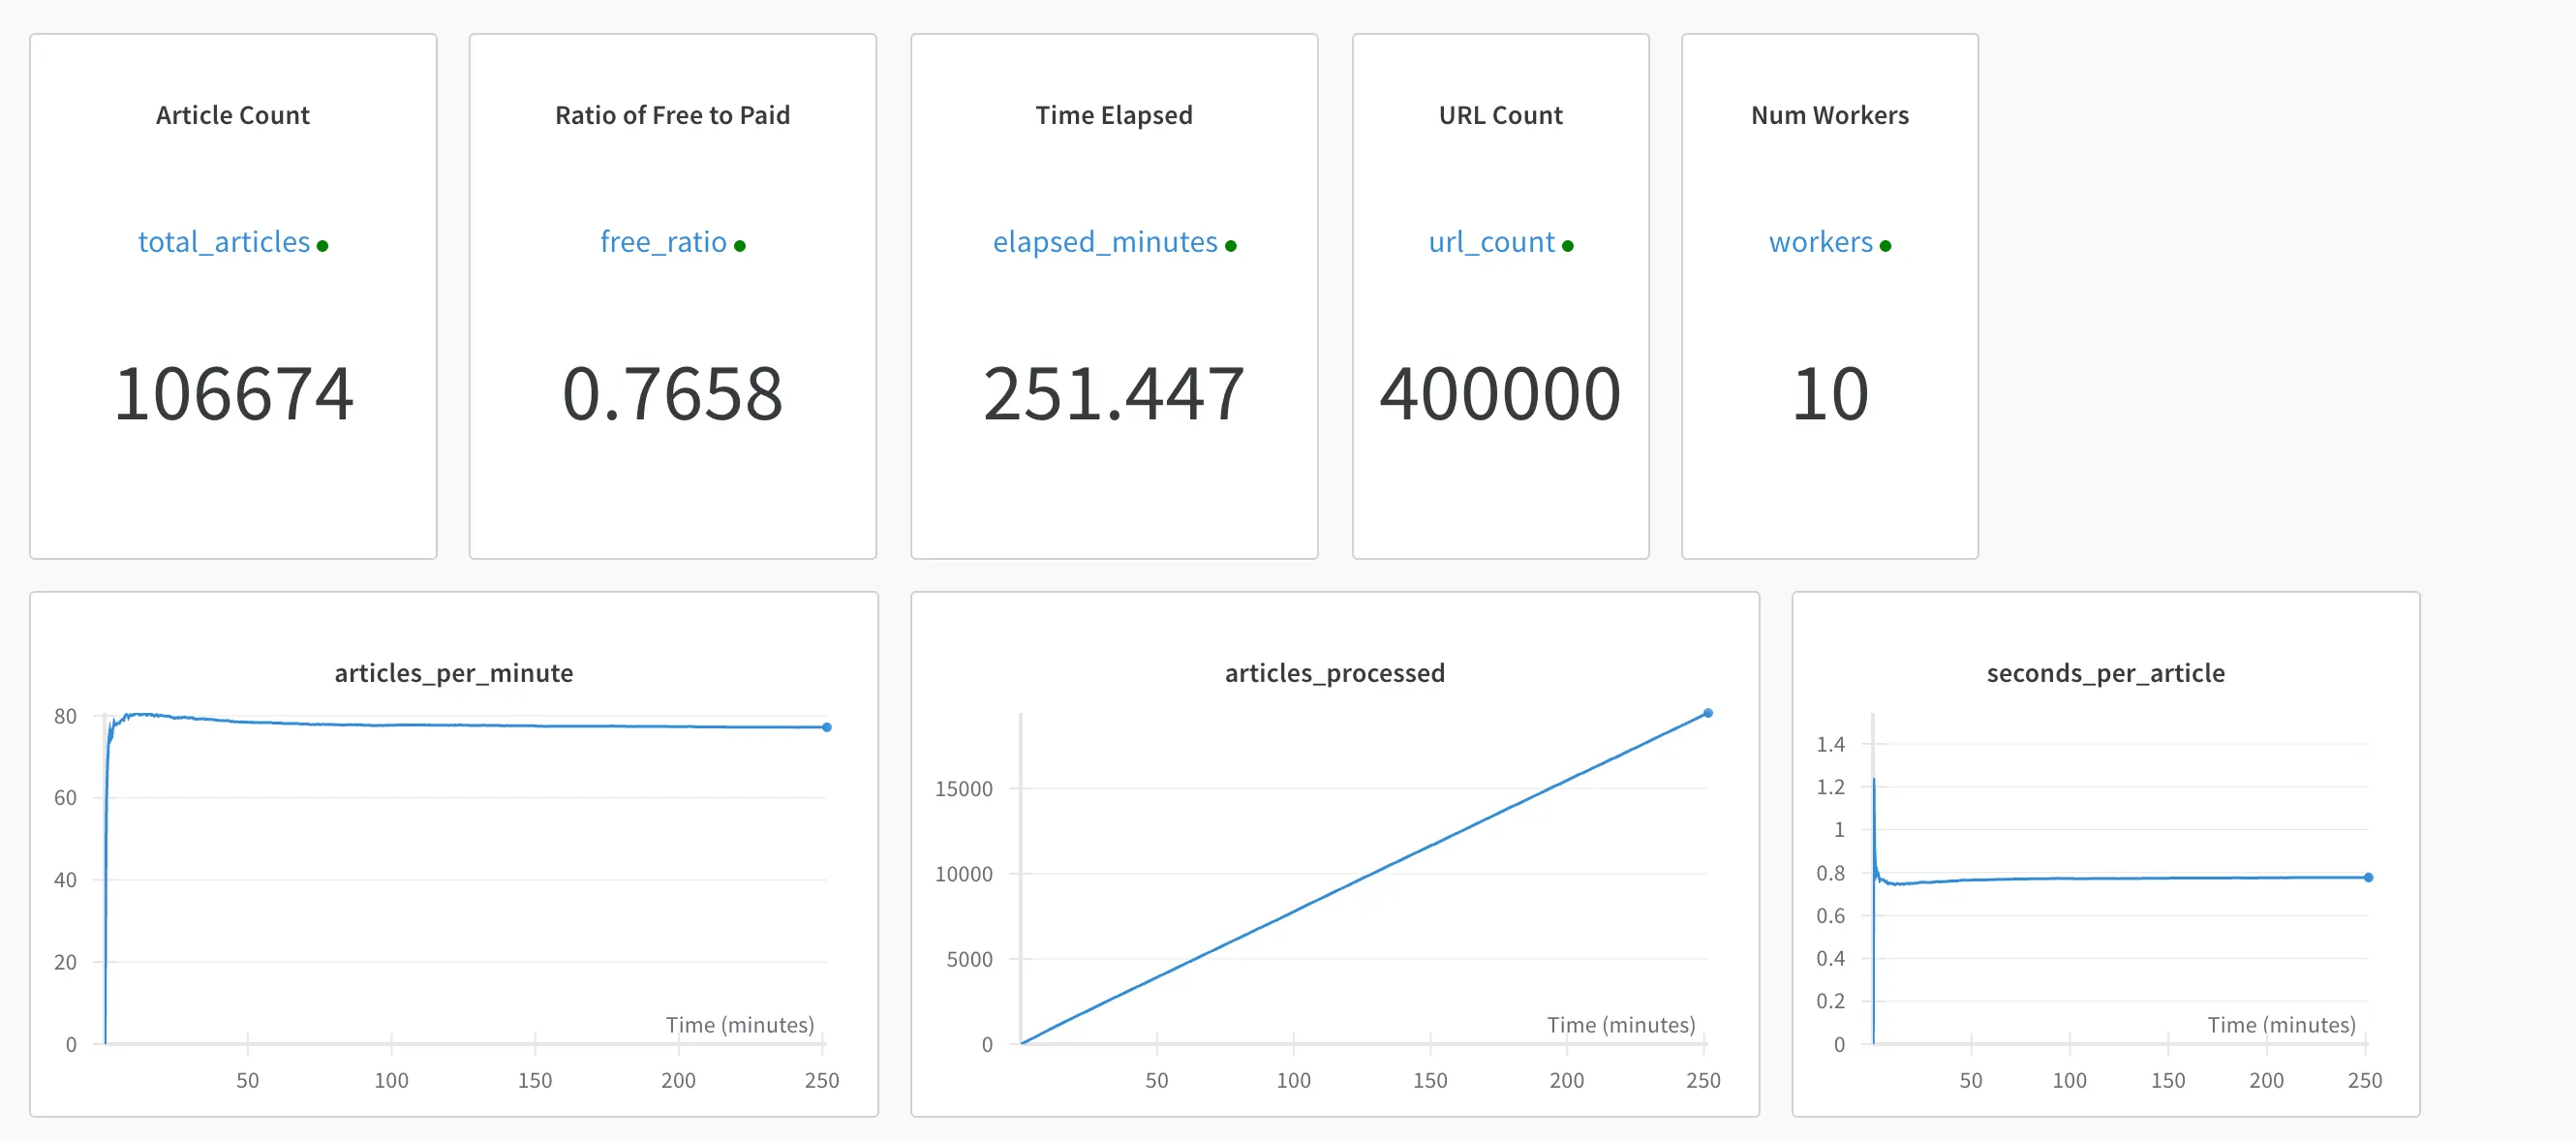
\includegraphics[width=0.6\textwidth]{images/weights_and_biases.png}
    \caption{Weights \& Biases dashboard summarizing worker throughput, error rates, and premium access metrics collected during scraping.}
    \label{fig:wandb_dashboard}
\end{figure}

\newpage

\section{Data Analysis}

\subsection{Dataset Overview}

Our initial scraping process, initiated from the 32 million URLs derived from the sitemaps, culminated in a raw dataset of $\mathbf{65,248}$ fully scraped articles.

\subsubsection*{Ensuring a Fair Comparison}

Medium.com introduced the ability for paid memberships in early 2017. As we want to ensure comparability between free and paid articles, taking into account any articles published before this date would introduce a significant bias. Furthermore, to allow for sufficient adoption of the commercial plan by authors and stabilize publication patterns, we only consider articles published after the first of January 2020.

This filtering step resulted in a final analysis dataset of $\mathbf{33,510}$ articles published between January 2020 and May 2025, contributed by $\mathbf{24,639}$ unique authors, and containing a total of $\mathbf{83,064}$ responses.

Of this final, cleaned dataset, $\mathbf{33.6\%}$ ($\mathbf{11,262}$ articles) were classified as member-only (paid), and $\mathbf{56.5\%}$ ($\mathbf{22,248}$ articles) were free. This composition provides a strong basis for comparative statistical analysis. The primary data points successfully extracted for this analysis include the article's text, estimated reading time, clap count, response count, author follower count, and premium status.

In Figure {\ref{fig:articles_per_month}}, the adoption and proportion of paid articles within our sample over time is clearly visible. The chart shows the monthly distribution of our scraped articles, where the consistent and increasing proportion of paid articles (relative to free articles) confirms that the post-2020 filter successfully captured the period of active growth in Medium's monetization strategy.

\begin{figure}[H]
    \centering
    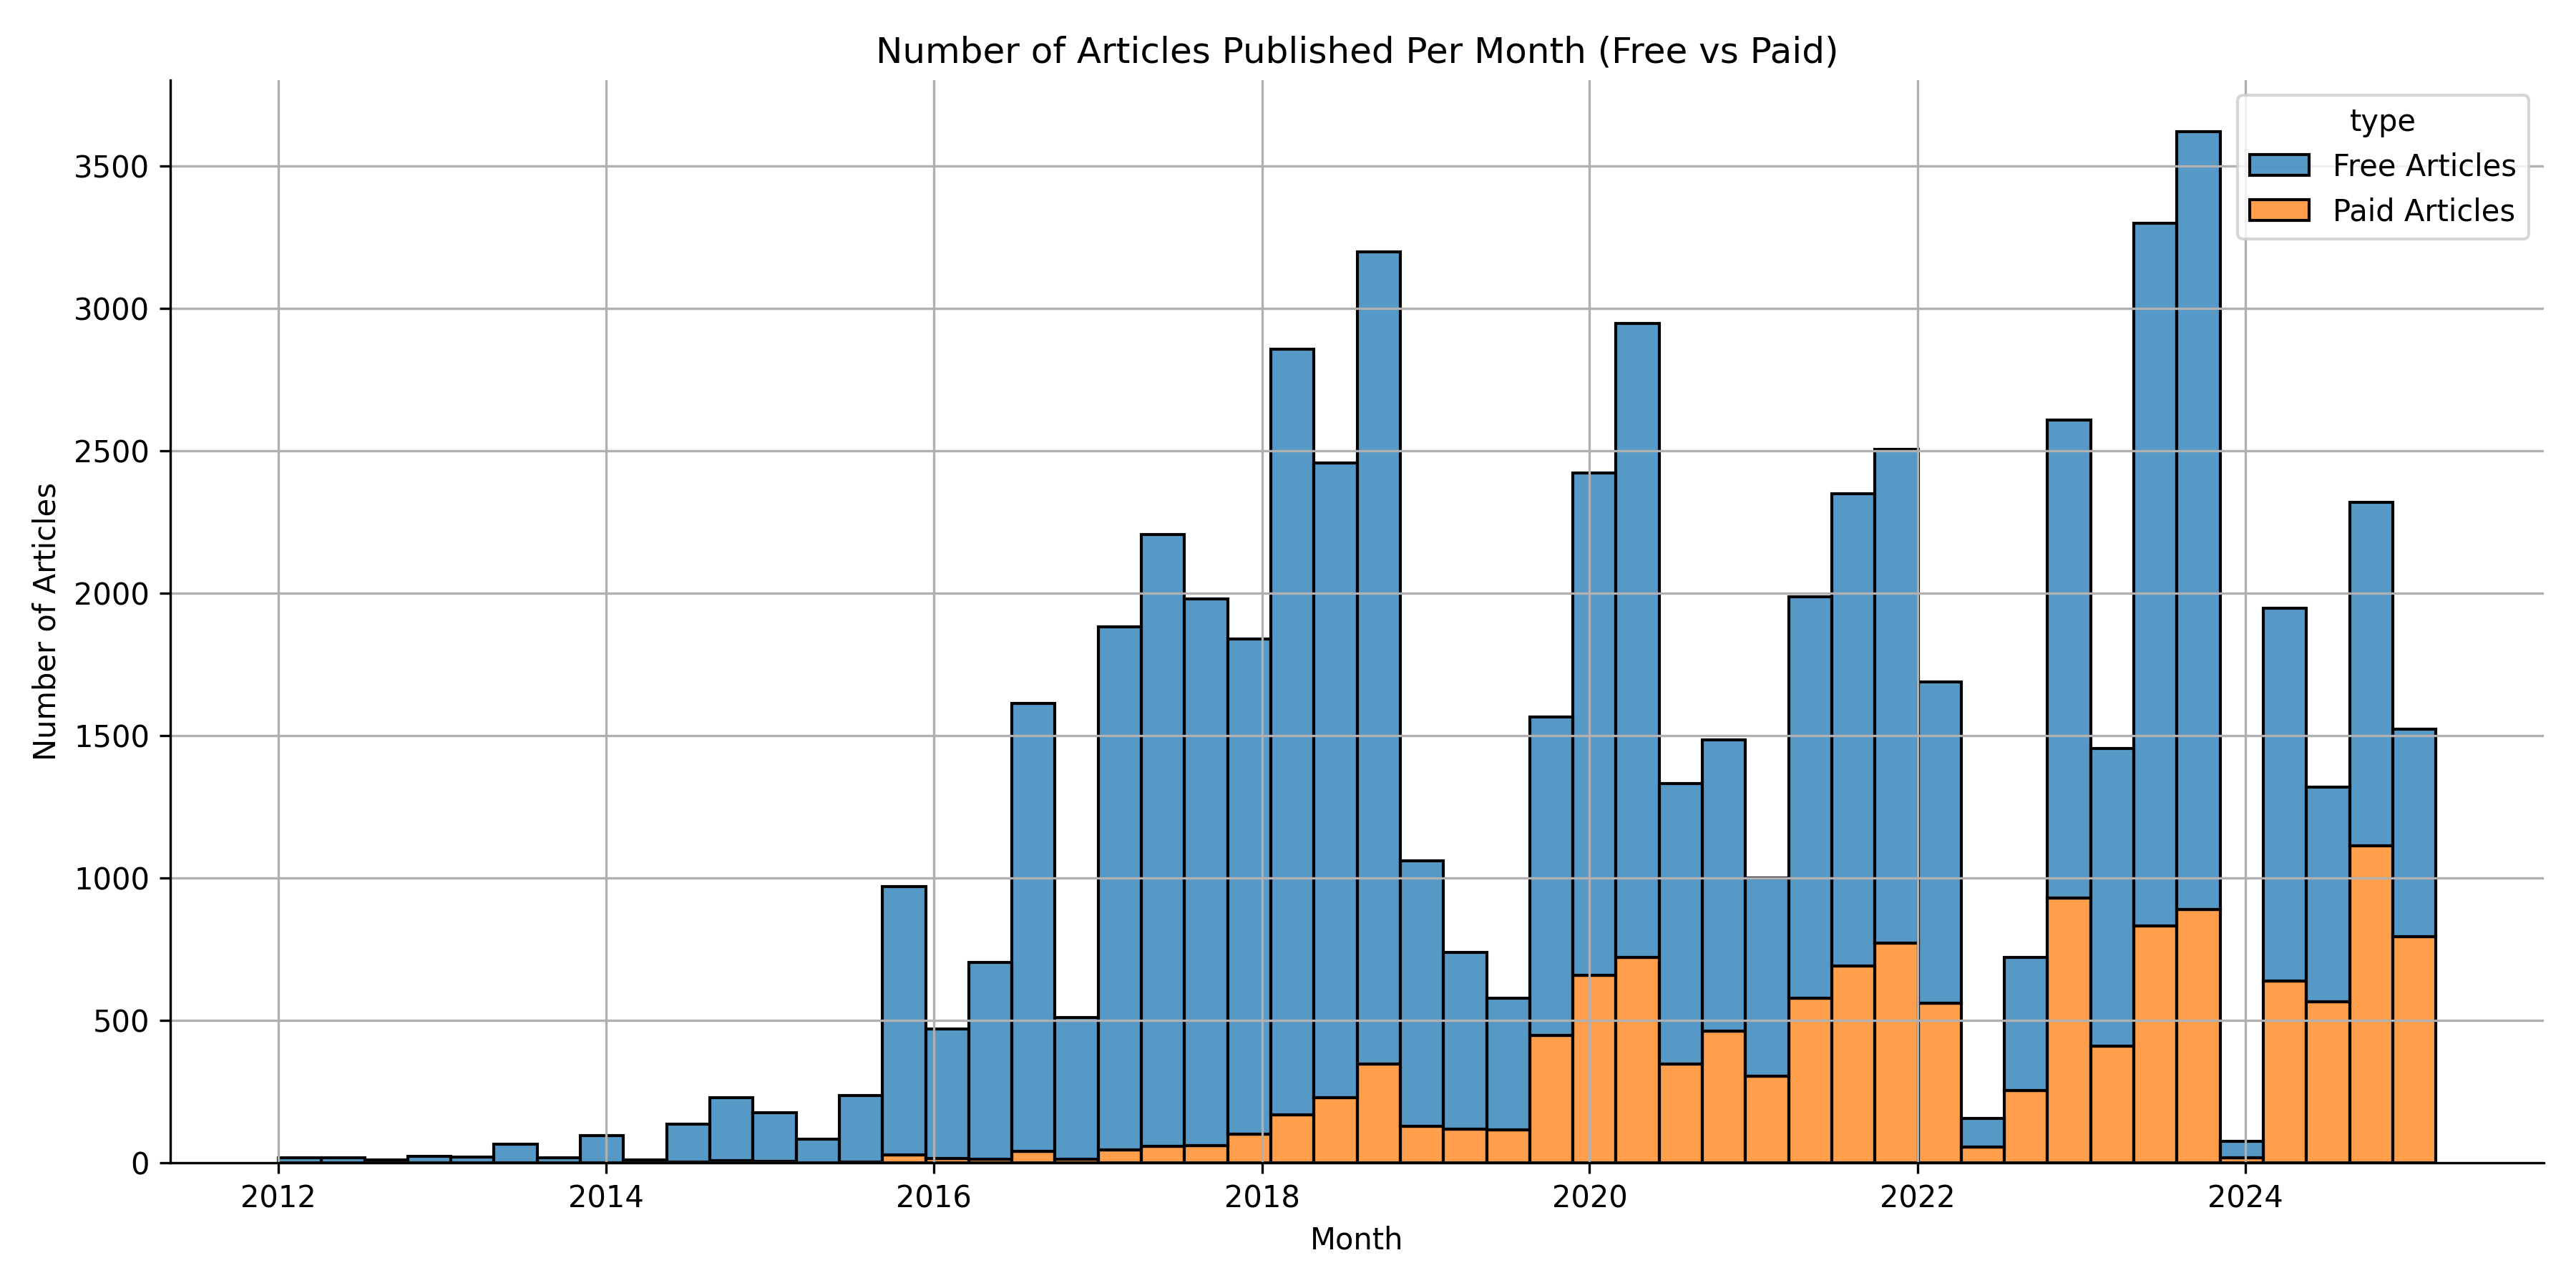
\includegraphics[width=0.7\textwidth]{images/articles_per_month.png}
    \caption{Distribution of scraped articles per month (2020-2025), segmented by premium status. The chart illustrates the growing relative proportion of member-only content in the dataset over time.}
    \label{fig:articles_per_month}
\end{figure}

\subsection{Comparative Statistics}

To quantify the differences in engagement and content length between member-only (paid) and free articles, we conducted a comparative statistical analysis. We focused on key metrics such as \todo{}.

\subsubsection{Descriptive Statistics}

Table \ref{tab:descriptive_stats} presents the core descriptive statistics for the engagement and length metrics, segmented by the article's premium status. These statistics highlight a clear difference in average engagement, particularly in clap count, where paid articles appear to significantly outperform free articles.

\begin{table}[H]
    \centering
    \caption{Descriptive Statistics for Key Metrics (Post-Jan 2020)}
    \label{tab:descriptive_stats}
    \begin{tabular}{lrrrrr}
        \toprule
        \textbf{Metric} & \textbf{Status} & \textbf{N} & \textbf{Mean} & \textbf{Median} & \textbf{Std. Dev.} \\
        \midrule
        \textbf{Clap Count} & Paid & 11,262 & 407.9 & 207.0 & 519.0 \\
        & Free & 22,248 & 122.4 & 40.0 & 272.1 \\
        \midrule
        \textbf{Response Count} & Paid & 11,262 & 4.9 & 2.0 & 7.0 \\
        & Free & 22,248 & 1.2 & 0.0 & 3.1 \\
        \midrule
        \textbf{Reading Time (min)} & Paid & 11,262 & 6.0 & 5.0 & 2.9 \\
        & Free & 22,248 & 5.9 & 5.0 & 3.2 \\
        \bottomrule
    \end{tabular}
    \vspace{0.5em}
\end{table}

\subsubsection{Hypothesis Testing (Two-Sample t-tests)}

Due to the observed differences in mean engagement metrics and reading time, we performed independent two-sample t-tests to formally assess the statistical significance of these differences. Given the large sample sizes, the Central Limit Theorem allows us to proceed with t-tests despite the non-normality and heteroscedasticity of the underlying populations, focusing on differences in the sample means.

The null hypothesis ($H_0$) for each test is that there is no difference between the means of paid and free articles for a given metric ($\mu_{paid} = \mu_{free}$).

The results of the t-tests, presented in Table \ref{tab:t_test_results}, reveal statistically significant differences between paid and free articles for all examined metrics. For clap count and response count, the t-statistics exceed 50, with p-values effectively at zero, indicating extremely strong evidence against the null hypothesis of no difference in means. This suggests that paid articles have substantially higher levels of engagement compared to free articles. Conversely, for reading time, the t-statistic of 2.26 yields a p-value of 0.0235, which, while below the conventional 0.05 threshold, indicates a marginally significant difference, implying that paid articles are, on average, slightly longer in reading time than free ones. These findings underscore the potential impact of premium status on content engagement and length within the Medium.com ecosystem.

\begin{table}[H]
    \centering
    \caption{Two-Sample T-Test Results for Key Metrics}
    \label{tab:t_test_results}
    \begin{tabular}{lrr}
        \toprule
        \textbf{Metric} & \textbf{t-statistic} & \textbf{p-value} \\
        \midrule
        Clap Count & 54.690392 & < 0.001 \\
        Response Count & 53.863954 & < 0.001 \\
        Reading Time (min) & 2.264893 & 0.023528 \\
        \bottomrule
    \end{tabular}
\end{table}

\todo{maybe extend this part?}

\subsection{Topic Modeling}

\subsubsection{Introduction}

Topic modeling using embeddings represents a modern approach to uncovering thematic structures in text data, leveraging dense vector representations to capture semantic similarities. Unlike traditional methods like Latent Dirichlet Allocation (LDA), embedding-based techniques utilize pre-trained language models to generate contextual embeddings, allowing for more nuanced topic discovery that accounts for word polysemy and context.

In our analysis of Medium.com articles, we employ embedding-based topic modeling to compare thematic distributions between paid and free content. This method enables us to identify clusters of semantically similar articles and assess whether premium content exhibits distinct topical patterns compared to free articles.

\subsubsection{Data Preprocessing}

Preprocessing for embedding-based topic modeling involves standard text cleaning steps followed by embedding generation. We tokenize the article text, remove stopwords, and apply lemmatization to normalize the vocabulary. Short or low-quality articles are filtered out to ensure meaningful embeddings.

\todo{Detail the embedding model used (e.g., Sentence-BERT), preprocessing specifics, and any dimensionality reduction techniques applied to the embeddings.}

\subsubsection{Methodology}

We utilize BERTopic, a topic modeling framework that combines transformer-based embeddings with clustering algorithms. The process involves:
\begin{enumerate}
    \item Generating sentence-level or document-level embeddings using a pre-trained model
    \item Reducing dimensionality with techniques like UMAP
    \item Clustering embeddings using HDBSCAN
    \item Extracting representative topics using class-based TF-IDF
\end{enumerate}

\todo{Describe hyperparameters (e.g., embedding model, clustering parameters), training process, and evaluation metrics used for topic quality assessment.}

\subsubsection{Results}

\subsubsection{Results}

The embedding-based topic modeling using BERTopic identified 26 distinct topics across the dataset. We analyzed the proportion of paid articles within each topic and performed two-sample t-tests to assess if these proportions differ significantly from the overall paid proportion (33.6\%).

Table \ref{tab:topic_proportions} summarizes the mean proportion of paid articles per topic, along with t-statistics and p-values. Significant differences (p < 0.05) indicate over- or under-representation of paid content.

\begin{figure}[H]
    \centering
    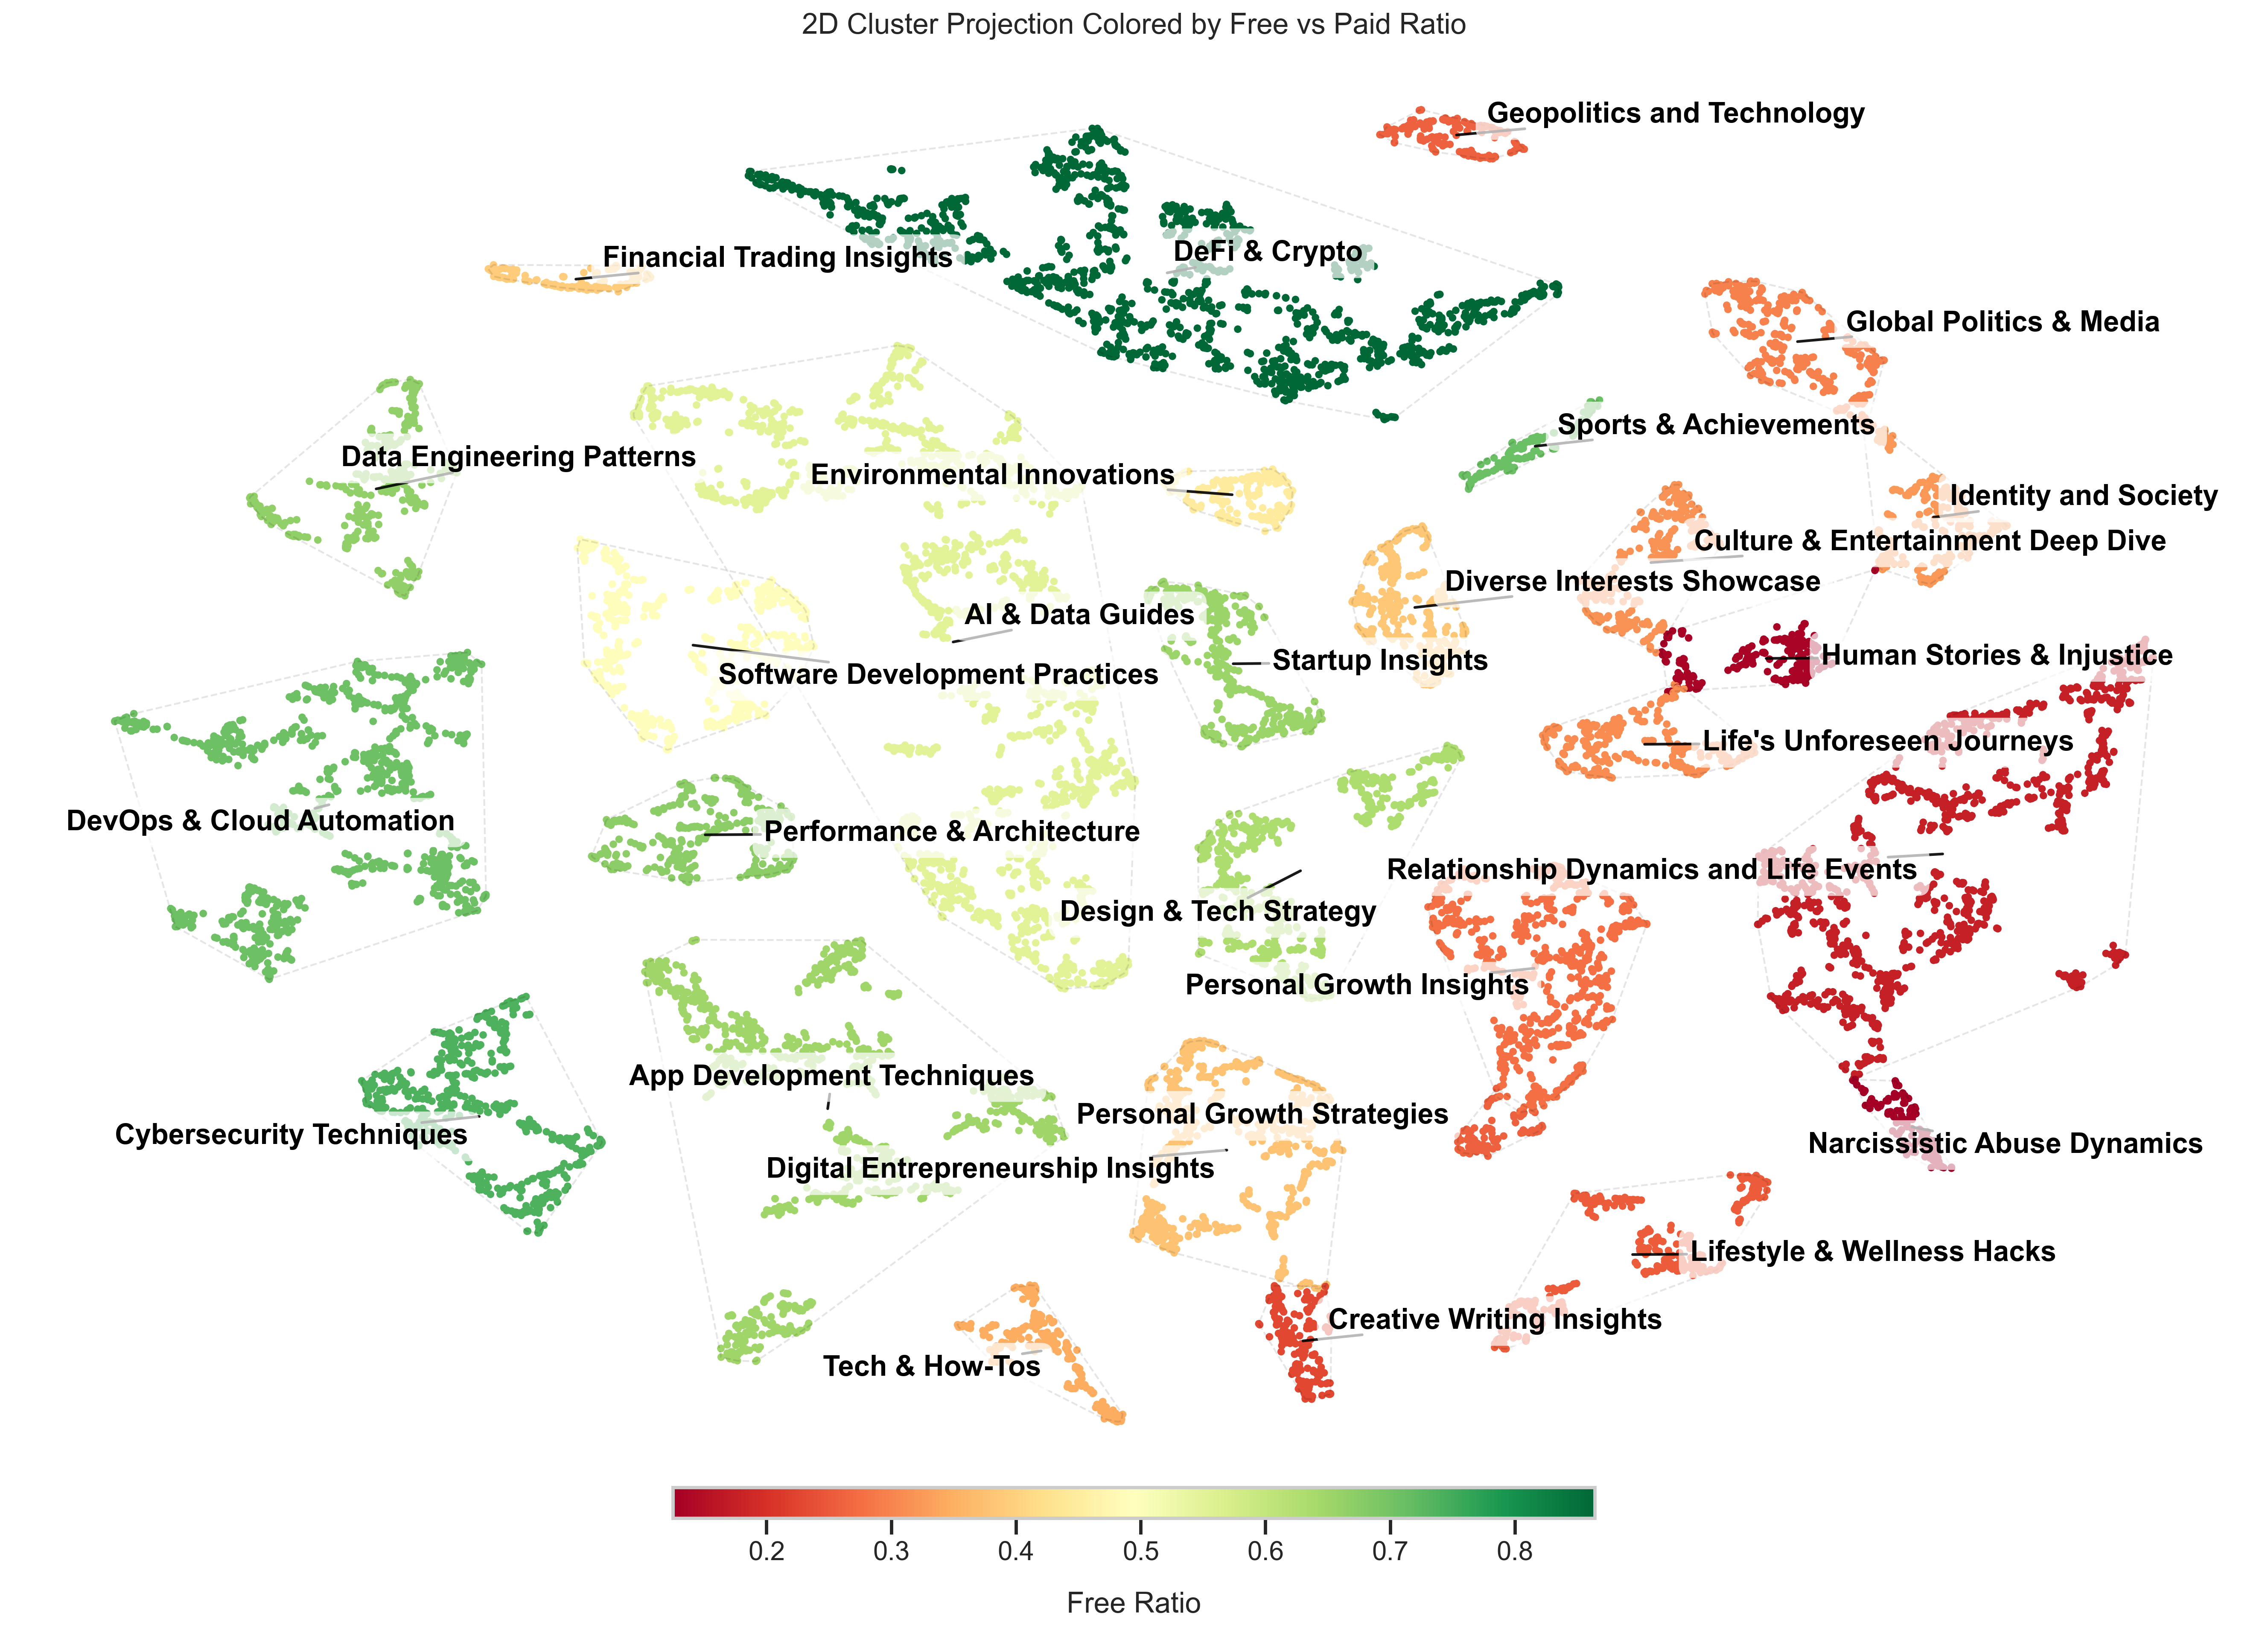
\includegraphics[width=\textwidth]{images/2D_Cluster_Free_Paid_Ratio.png}
    \caption{2D visualization of topic clusters showing free-to-paid article ratios. Color gradient (red to green) indicates free article proportion: red for lower free ratios (more paid), green for higher.}
    \label{fig:2d_clusters}
\end{figure}

\begin{table}[H]
    \centering
    \caption{Proportion of Paid Articles per Topic with Cluster Size and T-Test Results}
    \label{tab:topic_proportions}
    \begin{tabular}{lrrrr}
        \toprule
        \textbf{Topic} & \textbf{Size} & \textbf{Mean} & \textbf{t-statistic} & \textbf{p-value} \\
        \midrule
        DeFi \& Crypto & \textbf{1523} & \textbf{0.864} & \textbf{24.065} & \textbf{0.000} \\
        Cybersecurity Techniques & \textbf{579} & \textbf{0.737} & \textbf{4.633} & \textbf{0.000} \\
        Sports \& Achievements & 162 & 0.710 & 1.599 & 0.112 \\
        DevOps \& Cloud Automation & \textbf{1014} & \textbf{0.708} & \textbf{3.878} & \textbf{0.000} \\
        Performance \& Architecture & 379 & 0.673 & 0.834 & 0.405 \\
        Data Engineering Patterns & 424 & 0.665 & 0.540 & 0.589 \\
        Startup Insights & 393 & 0.654 & 0.052 & 0.958 \\
        App Development Techniques & 1087 & 0.649 & -0.221 & 0.825 \\
        Tech Strategy & 603 & 0.632 & -1.061 & 0.289 \\
        AI \& Data Guides & \textbf{1971} & \textbf{0.551} & \textbf{-9.075} & \textbf{0.000} \\
        Software Development Practices & \textbf{611} & \textbf{0.489} & \textbf{-8.070} & \textbf{0.000} \\
        Environmental Innovations & \textbf{204} & \textbf{0.446} & \textbf{-5.922} & \textbf{0.000} \\
        Financial Trading Insights & \textbf{153} & \textbf{0.392} & \textbf{-6.579} & \textbf{0.000} \\
        Diverse Interests Showcase & \textbf{337} & \textbf{0.383} & \textbf{-10.178} & \textbf{0.000} \\
        Digital Entrepreneurship Insights & \textbf{631} & \textbf{0.379} & \textbf{-14.174} & \textbf{0.000} \\
        Tech \& How-Tos & \textbf{257} & \textbf{0.346} & \textbf{-10.303} & \textbf{0.000} \\
        Identity and Society & \textbf{284} & \textbf{0.324} & \textbf{-11.818} & \textbf{0.000} \\
        Culture \& Entertainment Deep Dive & \textbf{311} & \textbf{0.318} & \textbf{-12.638} & \textbf{0.000} \\
        Life's Unforeseen Journeys & \textbf{304} & \textbf{0.309} & \textbf{-12.937} & \textbf{0.000} \\
        Global Politics \& Media & \textbf{348} & \textbf{0.296} & \textbf{-14.557} & \textbf{0.000} \\
        Personal Growth Insights & \textbf{691} & \textbf{0.276} & \textbf{-22.101} & \textbf{0.000} \\
        Personal Growth Strategies & \textbf{100} & \textbf{0.260} & \textbf{-8.908} & \textbf{0.000} \\
        Geopolitics and Technology & \textbf{170} & \textbf{0.259} & \textbf{-11.690} & \textbf{0.000} \\
        Lifestyle \& Wellness Hacks & \textbf{384} & \textbf{0.253} & \textbf{-18.020} & \textbf{0.000} \\
        Creative Writing Insights & \textbf{201} & \textbf{0.229} & \textbf{-14.268} & \textbf{0.000} \\
        Relationship Dynamics and Life Events & \textbf{1266} & \textbf{0.177} & \textbf{-44.341} & \textbf{0.000} \\
        Human Stories \& Injustice & \textbf{195} & \textbf{0.133} & \textbf{-21.280} & \textbf{0.000} \\
        Narcissistic Abuse Dynamics & \textbf{152} & \textbf{0.125} & \textbf{-19.607} & \textbf{0.000} \\
        \bottomrule
    \end{tabular}
\end{table}

\todo{Include visualizations like topic embeddings in 2D space, topic-word clouds, and comparative topic prevalence charts between paid and free content.}

The embedding-based model identified \todo{insert number} topics across the dataset. Topic distributions revealed \todo{key findings, such as prevalent topics in paid vs. free articles and semantic similarities}.

\todo{Include visualizations like topic embeddings in 2D space, topic-word clouds, and comparative topic prevalence charts between paid and free content.}

\subsubsection{Discussion}

The embedding-based topic modeling highlights \todo{insights into thematic differences between paid and free articles}. For example, paid articles may cluster around \todo{specific semantic themes}, while free content shows diversity in \todo{other areas}.

\todo{Discuss the advantages of embedding-based approaches over traditional methods, implications for content monetization, and limitations such as computational requirements or interpretability challenges.}


\section{AI Generated Content}


\section{Conclusion}

\todo{}

\end{document}